%%%%%%%%%%%%%%%%%%%%%%%%%%%%%%%%%%%%%%%%%
% Stylish Article
% LaTeX Template
% Version 2.1 (1/10/15)
%
% This template has been downloaded from:
% http://www.LaTeXTemplates.com
%
% Original author:
% Mathias Legrand (legrand.mathias@gmail.com) 
% With extensive modifications by:
% Vel (vel@latextemplates.com)
%
% License:
% CC BY-NC-SA 3.0 (http://creativecommons.org/licenses/by-nc-sa/3.0/)
%
%%%%%%%%%%%%%%%%%%%%%%%%%%%%%%%%%%%%%%%%%

%----------------------------------------------------------------------------------------
%	PACKAGES AND OTHER DOCUMENT CONFIGURATIONS
%----------------------------------------------------------------------------------------

\documentclass[fleqn,10pt]{SelfArx} % Document font size and equations flushed left

\usepackage[english]{babel} % Specify a different language here - english by default

\usepackage{lipsum} % Required to insert dummy text. To be removed otherwise

\captionsetup[figure]{justification=justified, singlelinecheck=off} 
\captionsetup[table]{justification=justified, singlelinecheck=off} 

%----------------------------------------------------------------------------------------
%	COLUMNS
%----------------------------------------------------------------------------------------

\setlength{\columnsep}{0.55cm} % Distance between the two columns of text
\setlength{\fboxrule}{0.75pt} % Width of the border around the abstract
\linespread{1.5}

%----------------------------------------------------------------------------------------
%	COLORS
%----------------------------------------------------------------------------------------

\definecolor{color1}{RGB}{0,0,90} % Color of the article title and sections
\definecolor{color2}{RGB}{10,20,20} % Color of the boxes behind the abstract and headings
\definecolor{xsubj}{RGB}{243,194,68} 
\definecolor{xsess}{RGB}{53,99,161} 
\definecolor{xsamp}{RGB}{18,165,121} 

%----------------------------------------------------------------------------------------
%	HYPERLINKS
%----------------------------------------------------------------------------------------

\usepackage{hyperref} % Required for hyperlinks
\hypersetup{hidelinks,colorlinks,breaklinks=true,urlcolor=color2,citecolor=color1,linkcolor=color1,bookmarksopen=false,pdftitle={Title},pdfauthor={Author}}
%----------------------------------------------------------------------------------------
%	ARTICLE INFORMATION
%----------------------------------------------------------------------------------------

% \JournalInfo{Journal, Vol. XXI, No. 1, 1-5, 2013} % Journal information
\JournalInfo{$ $ } % Journal information
\Archive{Pre-print} % Additional notes (e.g. copyright, DOI, review/research article)

\PaperTitle{Numerical Instabilities in Analytical Pipelines Lead to Large and Meaningful Variability in Brain Networks} % Article title

\Authors{Gregory Kiar\textsuperscript{1}, Alan C. Evans\textsuperscript{1}, Tristan Glatard\textsuperscript{2}} % Authors
\affiliation{\textsuperscript{1}\textit{Montréal Neurological Institute, McGill University, Montréal, QC, Canada}}
\affiliation{\textsuperscript{2}\textit{Department of Computer Science and Software Engineering, Concordia University, Montréal, QC, Canada}}

\Keywords{Stability --- Network Neuroscience --- Neuroimaging --- Machine Learning --- Generalizability} % Keywords - if you don't want any simply remove all the text between the curly brackets
\newcommand{\keywordname}{Keywords} % Defines the keywords heading name

%----------------------------------------------------------------------------------------
%	ABSTRACT
%----------------------------------------------------------------------------------------

\Abstract{Machine learning models are commonly applied to human brain imaging datasets in an effort to associate
function or structure with behaviour, health, or other individual attributes. Such models often rely on low-dimensional
maps relating brain regions, generated by complex processing pipelines. However, the numerical instabilities inherent
to pipelines limits the fidelity of these estimates, and results in bias-rich derivatives serving as inputs to these
machine learning models. This work seeks to take advantage of numerical instabilities in pipelines towards reducing the
bias in networks used by machine learning models. We found that resampling brain networks across a series of
numerically perturbed outcomes led to more consistently generalizable performance in all tested classifiers,
preprocessing strategies, and dimensionality reduction techniques when tasked with an age classification task.
Importantly, this finding does not hinge on a large number of perturbed networks in order to exhibit improved
performance, suggesting that even minimally perturbing a dataset reduces bias in the resulting models.}


%----------------------------------------------------------------------------------------

\begin{document}

\flushbottom % Makes all text pages the same height
\maketitle % Print the title and abstract box
% \tableofcontents % Print the contents section
\thispagestyle{empty} % Removes page numbering from the first page

%----------------------------------------------------------------------------------------
%	ARTICLE CONTENTS
%----------------------------------------------------------------------------------------

\section*{Introduction}
words

\section*{Materials \& Methods}

The objective of this study was to evaluate the impact of aggregating collections of unstable brain networks towards
learning robust brain-phenotype relationships. We sampled and aggregated simulated networks within individuals to learn
relationships between brain connectivity and individual traits, and compared this to traditional, baseline, performance
on these tasks. We compared aggregation strategies with respect to baseline performance, the number of perturbed
samples, and the distribution of the target variables. Finally, we compared the aggregation of unstable derivatives to
aggregation obtained through the traditional acquisition of repeated measurements.

All developed software and analysis resources for this project have been made available through GitHub at
\url{https://github.com/gkpapers/2020AggregateMCA}.

\subsection*{Dataset}

An existing dataset containing Monte Carlo Arithmetic (MCA) perturbed structural human brain networks was used for
these experiments~\cite{Kiar2020-yz}. The perturbations introduced for the generation of brain networks in this dataset
were at the level of machine-error, simulating expected error over a typical pipeline execution. This dataset consists
of two distinct collections containing i) a single session of data from $100$ individuals (D100;
$100\times 1 \times1$), or ii) two sessions which have each been subsampled into two components from $25$ individuals
(D25; $25\times 2\times 2$). In both cases, the derived brain networks were generated with a probabilistic structural
connectome estimation pipeline~\cite{Garyfallidis2014-ql} using a fixed random seed, and MCA perturbations were added
to all Python-implemented operations throughout the pipeline. Each sample was simulated $20$ times, resulting in
$2,000$ unique graphs per dataset. Further information on the processing and curation of this dataset can be found
here~\cite{Garyfallidis2014-ql}.

While the D100 collection enabled the exploration of subsampling and aggregation methods in a typical learning context
for neuroimaging~\cite{Dimitriadis2017-pd,Buchanan2014-pm}, D25 allowed for both the evaluation of these techniques in
a small-sample setting and for their comparison to traditional approaches for data augmentation through repeated
measurement, either across session or subsampling.

As the target for classification, individual-level phenotypic data strongly implicated in brain connectivity was
desired. Participant age, which has consistently been shown to have a considerable impact on brain
connectivity~\cite{Meier2012-ve,Wu2012-uc,Bookheimer2019-ti,Zhao2015-rm}, was selected and turned into a binary target
by dividing participants into adult ($>18$) and non-adult groups (D100: $68\%$ adult, D25: $40\%$ adult).

\subsection*{Preprocessing}
The brain networks being used for classification were represented as symmetric $83 \times 83$ adjacency matrices. To
reduce redundancy in the data, all edges belonging to the upper-triangle of these matrices were preserved and
vectorized, resulting in a feature vector of $3,486$ edges per sample. All samples were preprocessed using one of four
standard techniques:

\paragraph{Raw} – The raw streamline count edge-weight intensities were used as originally calculated.

\paragraph{Log Transform} – The log10 of edge weights were taken, and edges with $0$ weight prior to the transform were
reset to $0$.

\paragraph{Rank Transform} – The edges were ranked based on their intensity, with the largest edge having the maximum
value. Ties were settled by averaging the rank, and all ranks were finally min-max scaled between $0$ and $1$.

\paragraph{Z-Score} – The edge weights were z-scored to have a mean intensity of $0$ and unit variance.

\subsection*{Machine Learning Pipelines}

The preprocessed connectomes were fed into pipelines consisting of two steps: dimensionality reduction, and
classification. Dimensionality reduction was applied using one of two methods:

\paragraph{Principal Component Analysis} – the connectomes were projected into the $20$ or $15$ dimensions of highest
variance for D100 and D25, respectively. The number of components was chosen to capture approximately $90\%$ of the
variance present within D100. This was reduced due to limitations in sample size when dividing D25 into training,
testing, and validation sets; approximately $85\%$ of variance was explained through $15$ components for D25.

\paragraph{Feature Agglomeration} – the number of features in each connectome were reduced by combining edges according
to maximum similarity/minimum variance using agglomerative clustering~\cite{Ward1963-uh}. The number of resulting
features was $20$ and $15$ for D100 and D25, respectively, to be consistent with the number of dimensions present after
PCA, above.

After dimensionality reduction, samples were fed into one of five distinct classifiers as implemented through scikit
learn~\cite{Pedregosa2011-uz}:

\paragraph{Support Vector Machine} – the model was fit using a radial basis function (RBF) kernel, L2 penalty, and a
balanced regularization parameter to account for uneven class membership.

\paragraph{Logistic Regression} – a linear solver was used due to the relatively small dataset size. L2 regularization
and balanced class weights were used, as above.

\paragraph{K-Nearest Neighbour} – class membership was determined using an L2 distance and the nearest $10\%$ of
samples.

\paragraph{Random Forest} – $100$ decision trees were fit using balanced class weights, each splitting the dataset
according to a maximum of $4$ or $3$ features per node for D100 and D25, respectively (corresponding to the square root
of $20$ and $15$).

\paragraph{AdaBoost} – a maximum of $50$ decision trees were fit sequentially such that sample weights were iteratively
adjusted to prioritize performance on previously incorrectly-classified samples, consistent with~\cite{Freund1997-qy}.

The hyperparameters for all models were refined from their default values to be appropriate for a small and imbalanced
dataset. The performance for all pipeline combinations of preprocessing methods, dimensionality reduction techniques,
and models using the reference (i.e. unperturbed) executions in the D100 dataset ranged from an F1 score of
$0.64 – 0.875$ with a mean of $0.806$; this evaluation was performed on a consistent held-out test set which was used
for all experiments, as described in a following section. This set of models was chosen as it includes i) well
understood standard techniques, ii) both parametric and non-parametric methods, iii) both ensemble and non-ensemble
methods, and iv) models which have been commonly deployed across neuroimaging datasets~\cite{Meier2012-ve,Tunc2016-cz,
Zhu2018-cs,Payabvash2019-tm,Crossley2014-tg,Park2015-uj,Nayak2016-wl,Tolan2018-nq}.

\subsection*{Dataset Sampling}

As a chief purpose of this manuscript involves the comparison of various forms of aggregation across simulated pipeline
outputs, the datasets and classifiers were sampled, evaluated, and combined according to the following procedures:

\paragraph{Reference} – networks generated without any MCA perturbations were selected for input to the models, serving
as a benchmark. For the repeated measures evaluation using D25, a single observation (first session, first subsample)
per individual was selected.

\paragraph{Jackknife} – the datasets were repeatedly sampled such that a single randomly chosen observation of each
unique network was selected (i.e. derived from the same input datum). This resampling was performed $100$ times in the
case of MCA simulation experiments for both D100 and D25, and $10$ times for repeated session or subsample experiments
on D25. In all cases, the number of resamplings was $5\times$ the number of unique observations per network, resulting
in a broad and overlapping sampling of the datasets.

\paragraph{Median} – the edgewise median of all observations of the same network were used as the samples for training
and evaluation. This method was not used in the D25 repeated measurement setting due to a small and even number of
samples.

\paragraph{Mean} – similar to the above, the edgewise mean of all observations for each network were computed and used
as input data to the classifiers in both collections.

\paragraph{Consensus} – a distance-dependent average network~\cite{Betzel2018-eo} was computed across all observations
of each network. This data-aware aggregation method, developed for structural brain network analysis, preserves network
properties often distorted when computing mean or median networks. This approach was not used in the D25 repeated
measurement setting, due to the small number of samples.

\paragraph{Mega-analysis} – all observations of each network were used simultaneously for classification. Samples were
organized such that all observations of the same network only appeared within a single fold for training and
evaluation, ensuring double-dipping was avoided.

\paragraph{Meta-analysis} – individual classifiers trained across jackknife dataset resamplings were treated as
independent models and aggregated into an ensemble classifier. The ensemble was fit using a logistic regression
classifier across the outputs of the jackknifed classifiers to learn a relationship between the predicted and true
class labels.

The robustness and possible benefit of each subsampling approach was measured by evaluation on a subset of all MCA
simulations, including $9$ distinct numbers of simulations, ranging from $20$ to $2$ simulations per sample. Combining
the dataset sampling methods, the set of simulations, preprocessing strategies, dimensionality reduction techniques,
and classifier models, there were $2,200$ and $2,520$ models trained and evaluated for D100 and D25, respectively.

\subsection*{Training \& Evaluation}

Prior to training models on the brain networks, $20\%$ of subjects were excluded from each dataset for use as an
out-of-sample test dataset for all experiments. With the remaining $80\%$ of subjects, cross validation was performed
following a stratified grouped $k$-fold approach ($k=5$). In this approach, samples were divided into training and
validation sets such that the target variable was proportionally represented on each side of the fold (stratified),
conditional upon all observations from the same individual or network falling upon the same side of the fold (grouped).
This resulted in $5$ fold-trained classifiers per configuration, each trained on $64\%$ of the samples and validated on
$16\%$, prior to each being tested on the remaining $20\%$ of held-out samples.

Classifiers were evaluated using F1 score, a standard measure for evaluating classification performance, especially in
an imbalanced setting. Performance on the test set was measured for each configuration both through the mean of each
fold-trained classifier and through a probability-based voting classifier. The voting classifier combined individual
estimators and made predictions based on the net probability of class membership, forming higher fidelity out-of-sample
predictions than any independent estimator. Importantly, this was done so that the trained estimators could be
meaningfully operationalized and applied to arbitrary new samples in practice. The performance of the voting classifier
was similarly evaluated through F1 score.


%------------------------------------------------
\section*{Results}
words

\subsection*{TODO: come up with result title}
\begin{figure*}[hbt]\centering
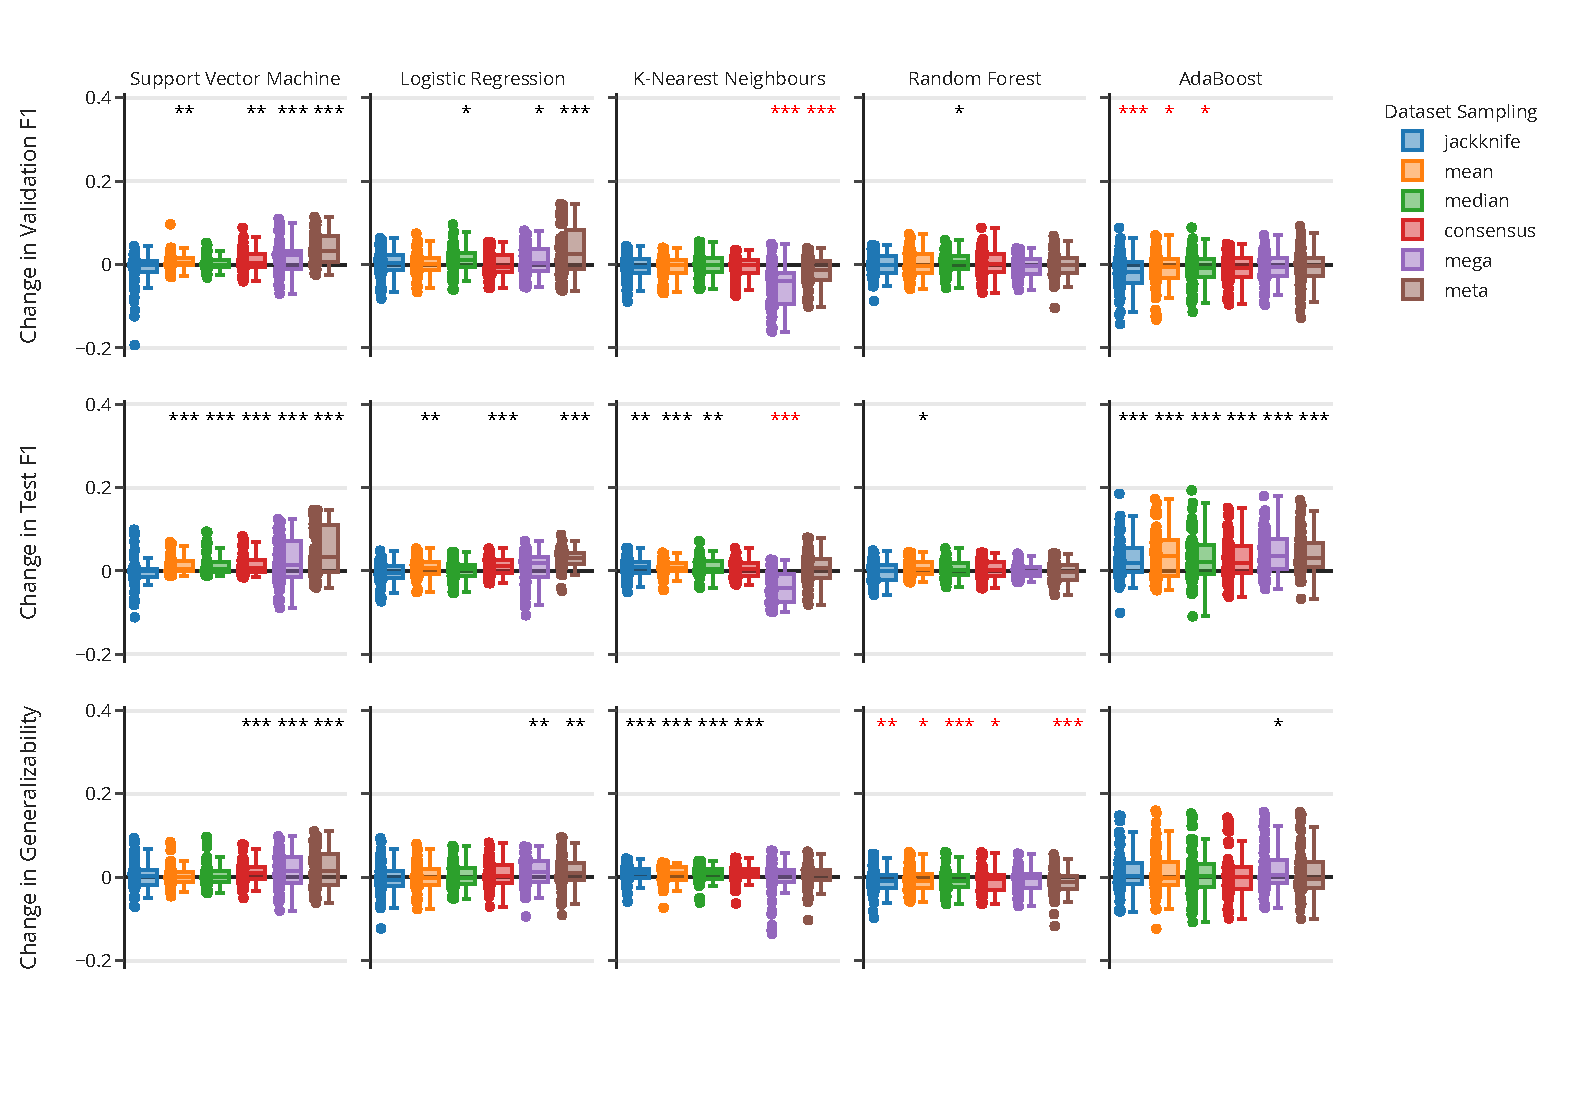
\includegraphics[width=\linewidth]{figures/1.pdf}
\caption{Relative change in classifier performance (F1 score) with respect to classifier type and dataset sampling
strategies as measured by performance on the validation set (top), test set (middle), as well as the generalizability
of performance across the two sets (bottom). Each data point represents performance from a single model, number of MCA
simulations, preprocessing strategy, and dimensionality reduction technique. Each star annotation indicates an order of
magnitude of statistically significant change in performance, with those in black or red indicating an increase or
decrease in performance, respectively. The baseline performance ranged from $0.66$ to $0.88$ across all models. This
figure shows that while support vector machine and logistic regression classifiers learn the validation set more
effectively, their improved performance fails to improve generalizability. In contrast, AdaBoost classifiers do not
improve on the validation set but form more generalizable predictions on the test set.}
\label{fig:overall_performance}
\end{figure*}

\subsection*{Data Resampling Increases the Predictability of Performance}
\begin{figure*}[bht!]\centering
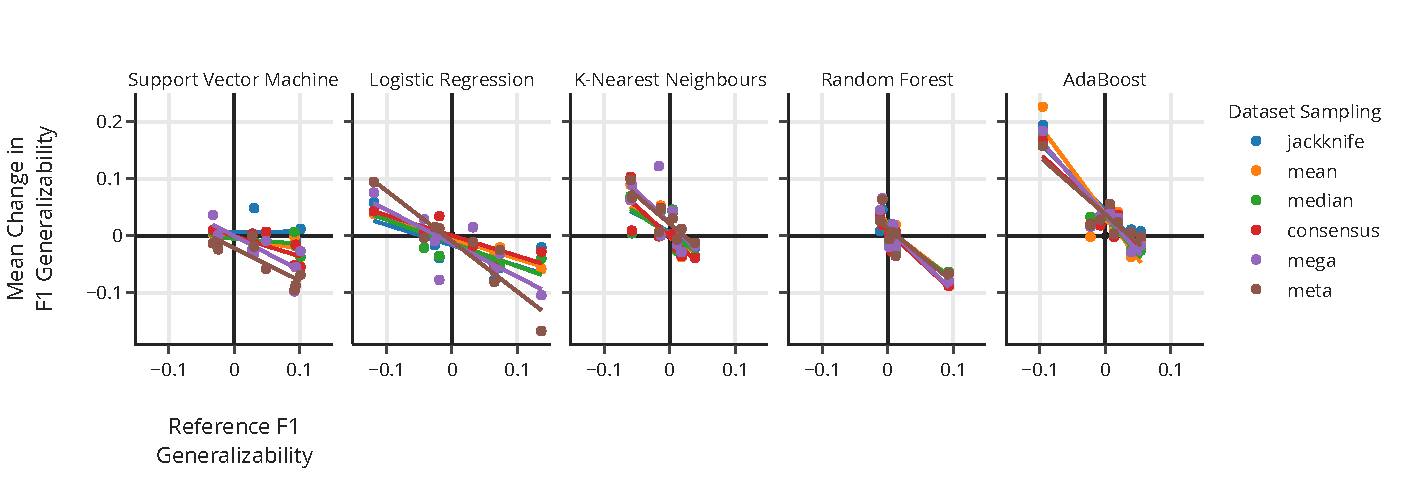
\includegraphics[width=\linewidth]{figures/2.pdf}
\caption{Change in the generalizability of classifiers with respect to the reference. Each data point represents the
mean change in generalizability for all models of the same type (i.e. preprocessing and dimensionality reduction) for a
given classifier and dataset sampling strategy. In order to have predictable performance on unseen samples, the target
generalizability is $0$, meaning that performance on the validation and testing set is equivalent. Models with negative
generalizability underperform, and those with positive generalizability overperform. This figure shows that
perturbation-enabled dataset resampling improves the generalizability of all models, shifting both underperforming and
overperforming models towards predictable performance.}
\label{fig:change_in_gen}
\end{figure*}


\subsection*{Data Resampling Benefit is Invariant To Number of Simulations}

\begin{figure*}[ht]\centering
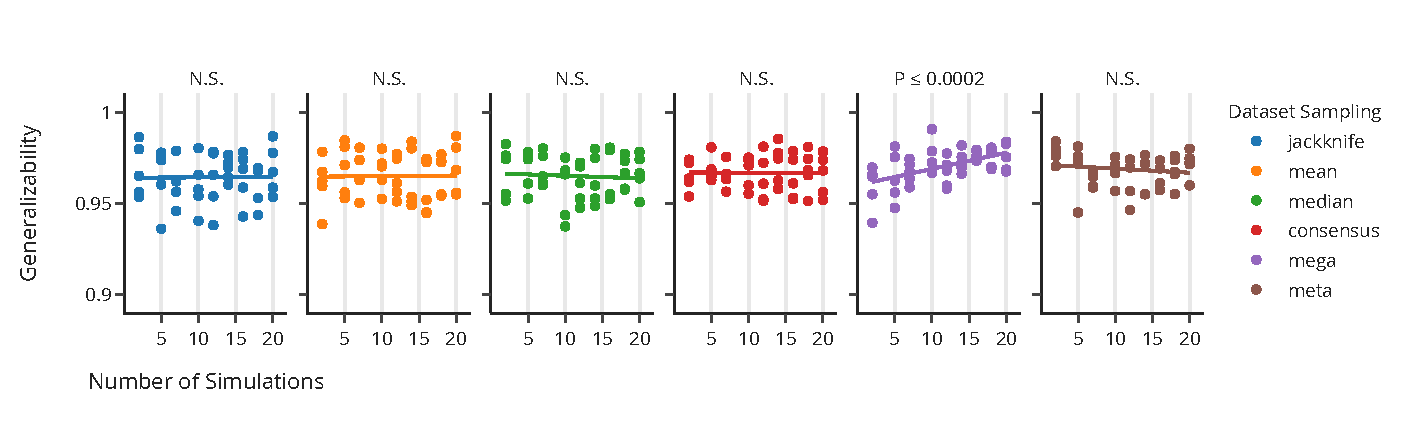
\includegraphics[width=\linewidth]{figures/3.pdf}
\caption{Variability in the performance of dataset sampling strategies with respect to the number of MCA simulations
used. Each number of simulations was sampled a single time, to avoid artificial skewing of the dataset due to the
inclusion of "more" or "less" meaningful samples; a single drawing of each split mimics a true perturbation experiment
context. This figure shows that while we previously noted an increase in the generalizability when resampling, there is
no relationship between the number of independent samples used and performance.}
\label{fig:nsamples}
\end{figure*}
 

\section*{Discussion}
- class imbalance... “Data is expensive, we don’t want to waste it, and biological oversampling (without a technique such as MCA) is hard… together, that’s why we went with balancing weights over undersampling”

- consider MCA as an oversampling technique which does not compromise the quality of samples or rely on interpolation in high dimensional data

- The first pass, we swept over both classifiers and targets, but I was lazy and didn’t make sure we had good performance, so results were all of high variance.

- The second pass, we made sure that we had good baseline performance in unique settings, but this required the addition of another degree of freedom through pre-processing, so the results when we mapped over all the combinations were still high variance and in some cases complete garbage.

- The third pass, we removed the degrees of freedom of target and classifier by fixing a single target to a single classifier. This led to better baseline performance for each task, but, of course, lead to the issue of not being able to actually draw conclusions on either target or classifier.

- For the fourth pass, I’m proposing to fix a single target, removing this degree of freedom entirely, but selecting one with both high performance and some variance across the set of classifiers used, so that we can model a relationship between model performance and impact of aggregation. If we wanted to extend this to other targets, too, I think we agree that it is useless to apply this on chance-classifiers; thus excluding BMI entirely, given the very high variance/generally weak relationship. Thus it would really only add sex to the mix, and wouldn’t particularly answer any questions about how consistent this is over other target variables, basically because “2 data points isn’t a trend”, despite complicating the picture further.

\subsection*{Data \& Code Availability}
The perturbed connectomes were publicly available data resource previously produced and made available by the
authors~\cite{Kiar2020-yz}. They can be found persistently at \url{https://doi.org/10.5281/zenodo.4041549}, and are
made available through The Canadian Open Neuroscience Platform (\url{https://portal.conp.ca/search}, search term
"Kiar"). All software developed for processing or evaluation is publicly available on GitHub at
\url{https://github.com/gkpapers/2020AggregateMCA}. Experiments were launched on Compute Canada's HPC cluster
environment. 

\subsection*{Author Contributions}
GK was responsible for the experimental design, data processing, analysis, interpretation, and the majority of writing.
All authors contributed to the revision of the manuscript. TG and ACE contributed to experimental design, analysis,
interpretation. The authors declare no competing interests for this work. Correspondence and requests for materials
should be addressed to Gregory Kiar at \url{gregory.kiar@mail.mcgill.ca}.

\subsection*{Acknowledgments} 
This research was financially supported by the Natural Sciences and Engineering Research Council of Canada (NSERC)
(award no. CGSD3-519497-2018). This work was also supported in part by funding provided by Brain Canada, in partnership
with Health Canada, for the Canadian Open Neuroscience Platform initiative.

%----------------------------------------------------------------------------------------
%	REFERENCE LIST
%----------------------------------------------------------------------------------------
% \phantomsection
\bibliographystyle{IEEEtran}
\bibliography{aggregating-unstable-derivatives}


\end{document}
